% !TEX root = thesis-ex.tex

The quark-gluon plasma is a state of matter that comprises of free partons and is formed in extreme conditions of temperature and pressure \cite{SHURYAK198071}.
First discovered in heavy ion collisions at the Relativistic Heavy Ion Collider (RHIC) \cite{ARSENE20051, Adcox:2004mh, ADAMS2005102, Back:2004je}, its study is motivated by the fact that is the only way to access the dynamics of partons that are otherwise confined within hadrons.


A schematic of a heavy ion collision is shown in Figure~\ref{fig:qgp_form}.
The colliding nuclei have a relativistic $\gamma$ factor of approximately 3000 and form discs.
As they collide, color fields from the partons within the colliding nuclei interact and fill the space between them.
The energy density in the collision depends on the number of colliding nucleons and the collision energy, and can range from 1 GeV/fm$^3$ for $\sqrtsnn = 7.7$ GeV at the lower limit of RHIC energies \cite{PhysRevC.93.024901} to 15 GeV/fm$^3$ for $\sqrtsnn = 5.02$ TeV at the Large Hadron Collider (LHC) \cite{PhysRevC.94.034903, PhysRevLett.109.152303, Jiang:2018wzu}.
This is well above the $0.2 - 1 \rm{GeV}/\rm{fm}^3$ energy density range required to form the QGP \cite{Karsch2002, PhysRevD.90.094503}.
After the collision the QGP cools and expands and the energy density between the receding nuclei starts to decrease.
At a certain critical temperature about 1-10 fm/c after the collision, the energy density decreases to lower than what is within a hadron, and the plasma forms a hadron gas \cite{doi:10.1146/annurev.nucl.46.1.71}.
This process, referred to as a chemical freeze-out, occurs at about 160 MeV \cite{Fodor_2004, ADAMS2005102, PhysRevC.93.024917, Borsanyi:2010bp}.
The hadrons within the gas have energies below the threshold for inelastic particle production but briefly scatter off of each other resulting in modifications to their momentum spectra.
This continues till the medium cools further and reaches what is called a thermal freeze-out at 100--150 MeV, at which point the hadrons fly freely towards the detector \cite{PhysRevC.69.024904, PhysRevC.72.014908, PhysRevC.75.024910, PhysRevC.88.044910}.

\begin{figure}[htbp]
\begin{center}
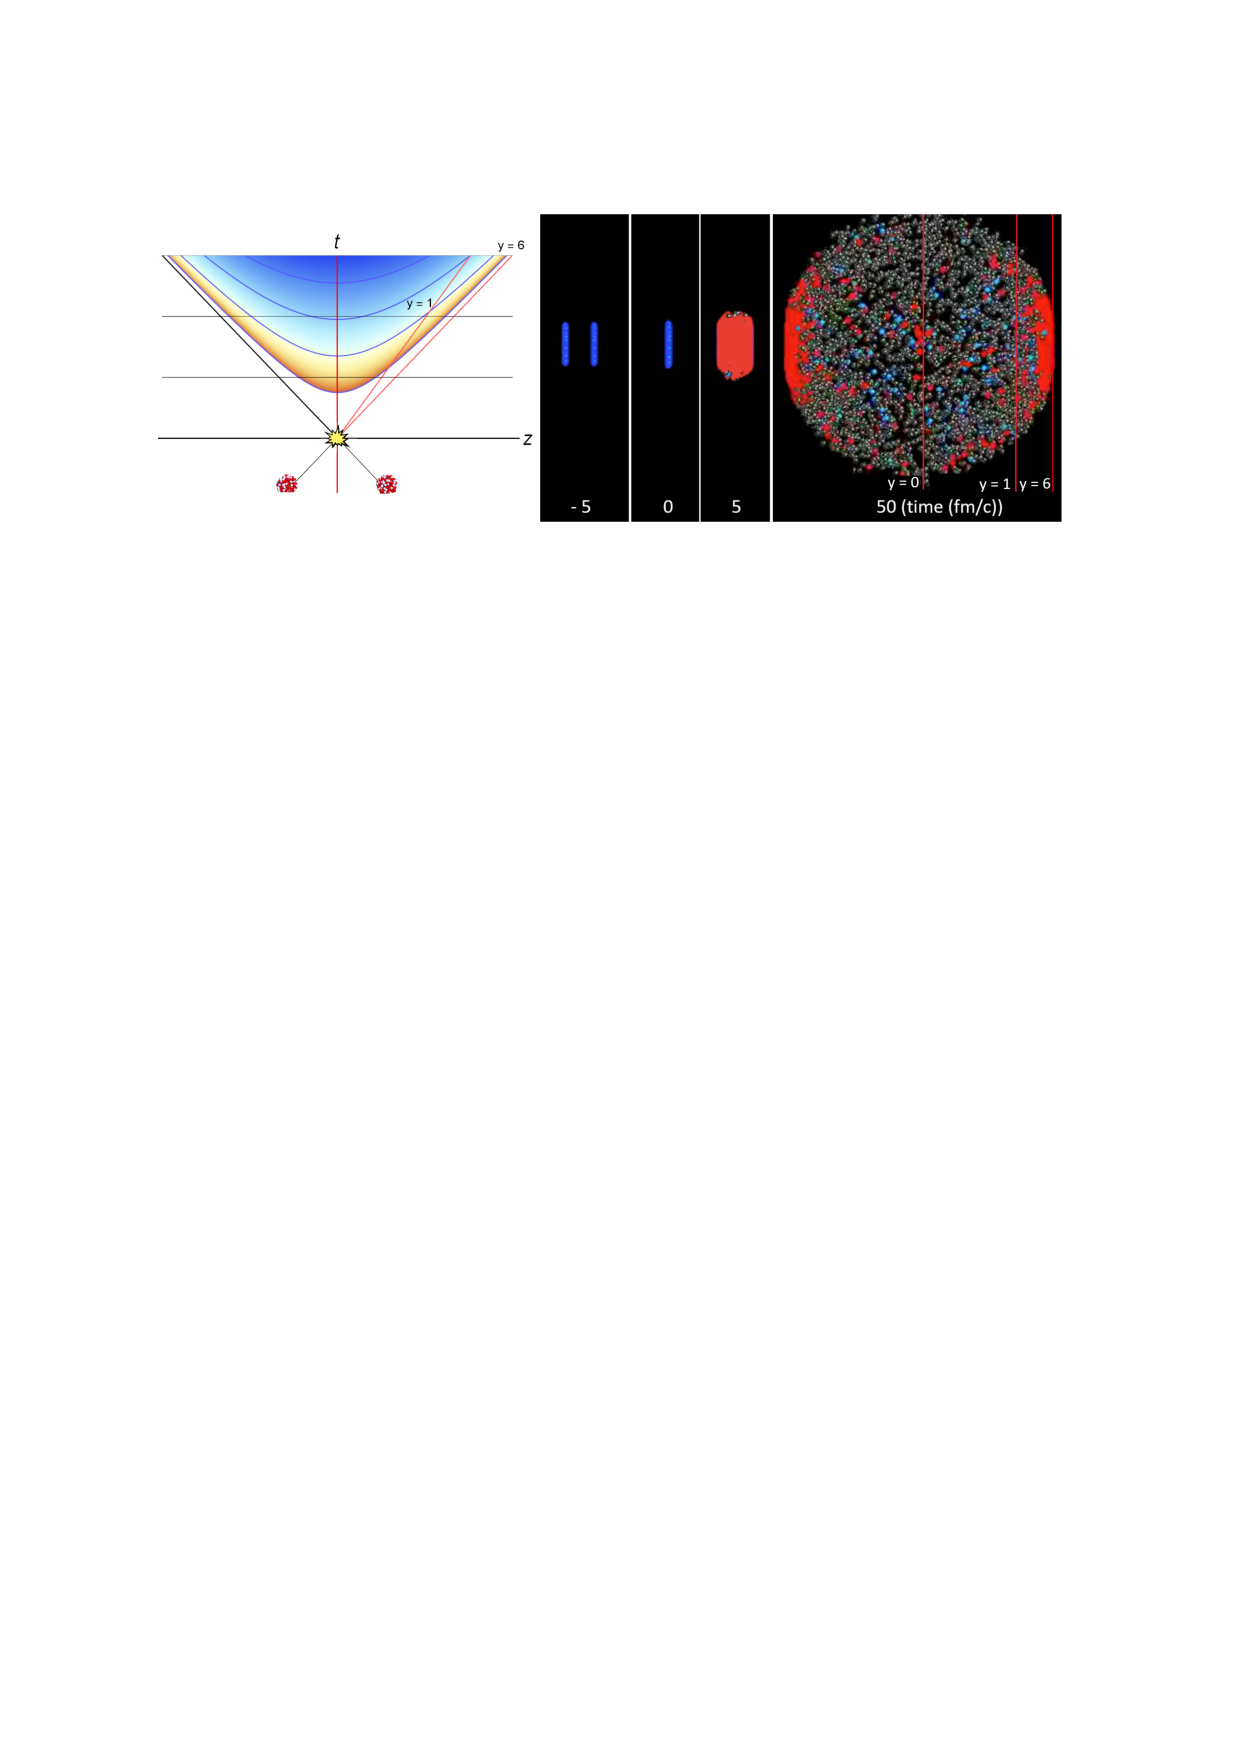
\includegraphics[width=0.85\textwidth]{figures/theory/qgp_formation}
\caption{(left) Space-time diagram for a heavy ion collision.
The color is indicative of the temperature of the QGP formed.
(right) Snapshots of a heavy ion collision at $\sqrtsnn = 2.76$ TeV at different times.
The Lorentz contracted nuclei are in blue while the QGP is in red.
Figure from Ref.~\cite{Busza:2018rrf}.}
\label{fig:qgp_form}
\end{center}
\end{figure}

It is important to note that the impact parameter of the colliding nuclei plays a significant role in the dynamics of the QGP that is formed.
This can be seen in Figure~\ref{fig:collision_centrality}, where the shape and size of the QGP produced for head-on (``central'') collisions is different from that in more glancing (``peripheral'') collisions.

The QGP was initially thought to be a weakly coupled parton gas because of asymptotic freedom from QCD.
The highly energetic collisions such as those at the LHC would imply weak interactions between the partons that make up the plasma \cite{PhysRevLett.34.1353, heinz2013collective, 10.1007/978-1-4020-2705-5_14}.
This would result in rare scatterings between the constituents of the hadron gas formed in such a collision, washing out any spatial anisotropies from the ``'lumpy''-ness of the colliding nuclei.
A strong coupling within the QGP however, would result in the pressure gradients in the medium and spatial anisotropies would be transformed to momentum anisotropies in the particles produced as shown in Figure~\ref{fig:overlap} \cite{Busza:2018rrf}.
In this picture, the non-uniform structure of the colliding nuclei would cause a momentum anisotropy \cite{Ster:1999ib} that would be further enhanced when looking at collisions that are less central and do not have perfect overlap between the colliding nuclei \cite{Poskanzer:1999ea, Pinkenburg:1999ya}.
These observations were seen in azimuthal correlation measurements implying that the medium is indeed strongly coupled \cite{Aaboud:2018ves, PhysRevLett.91.182301, Sirunyan:2017fts, PhysRevLett.116.132302}.

\begin{figure}
\centering
\begin{minipage}[b]{0.45\textwidth}
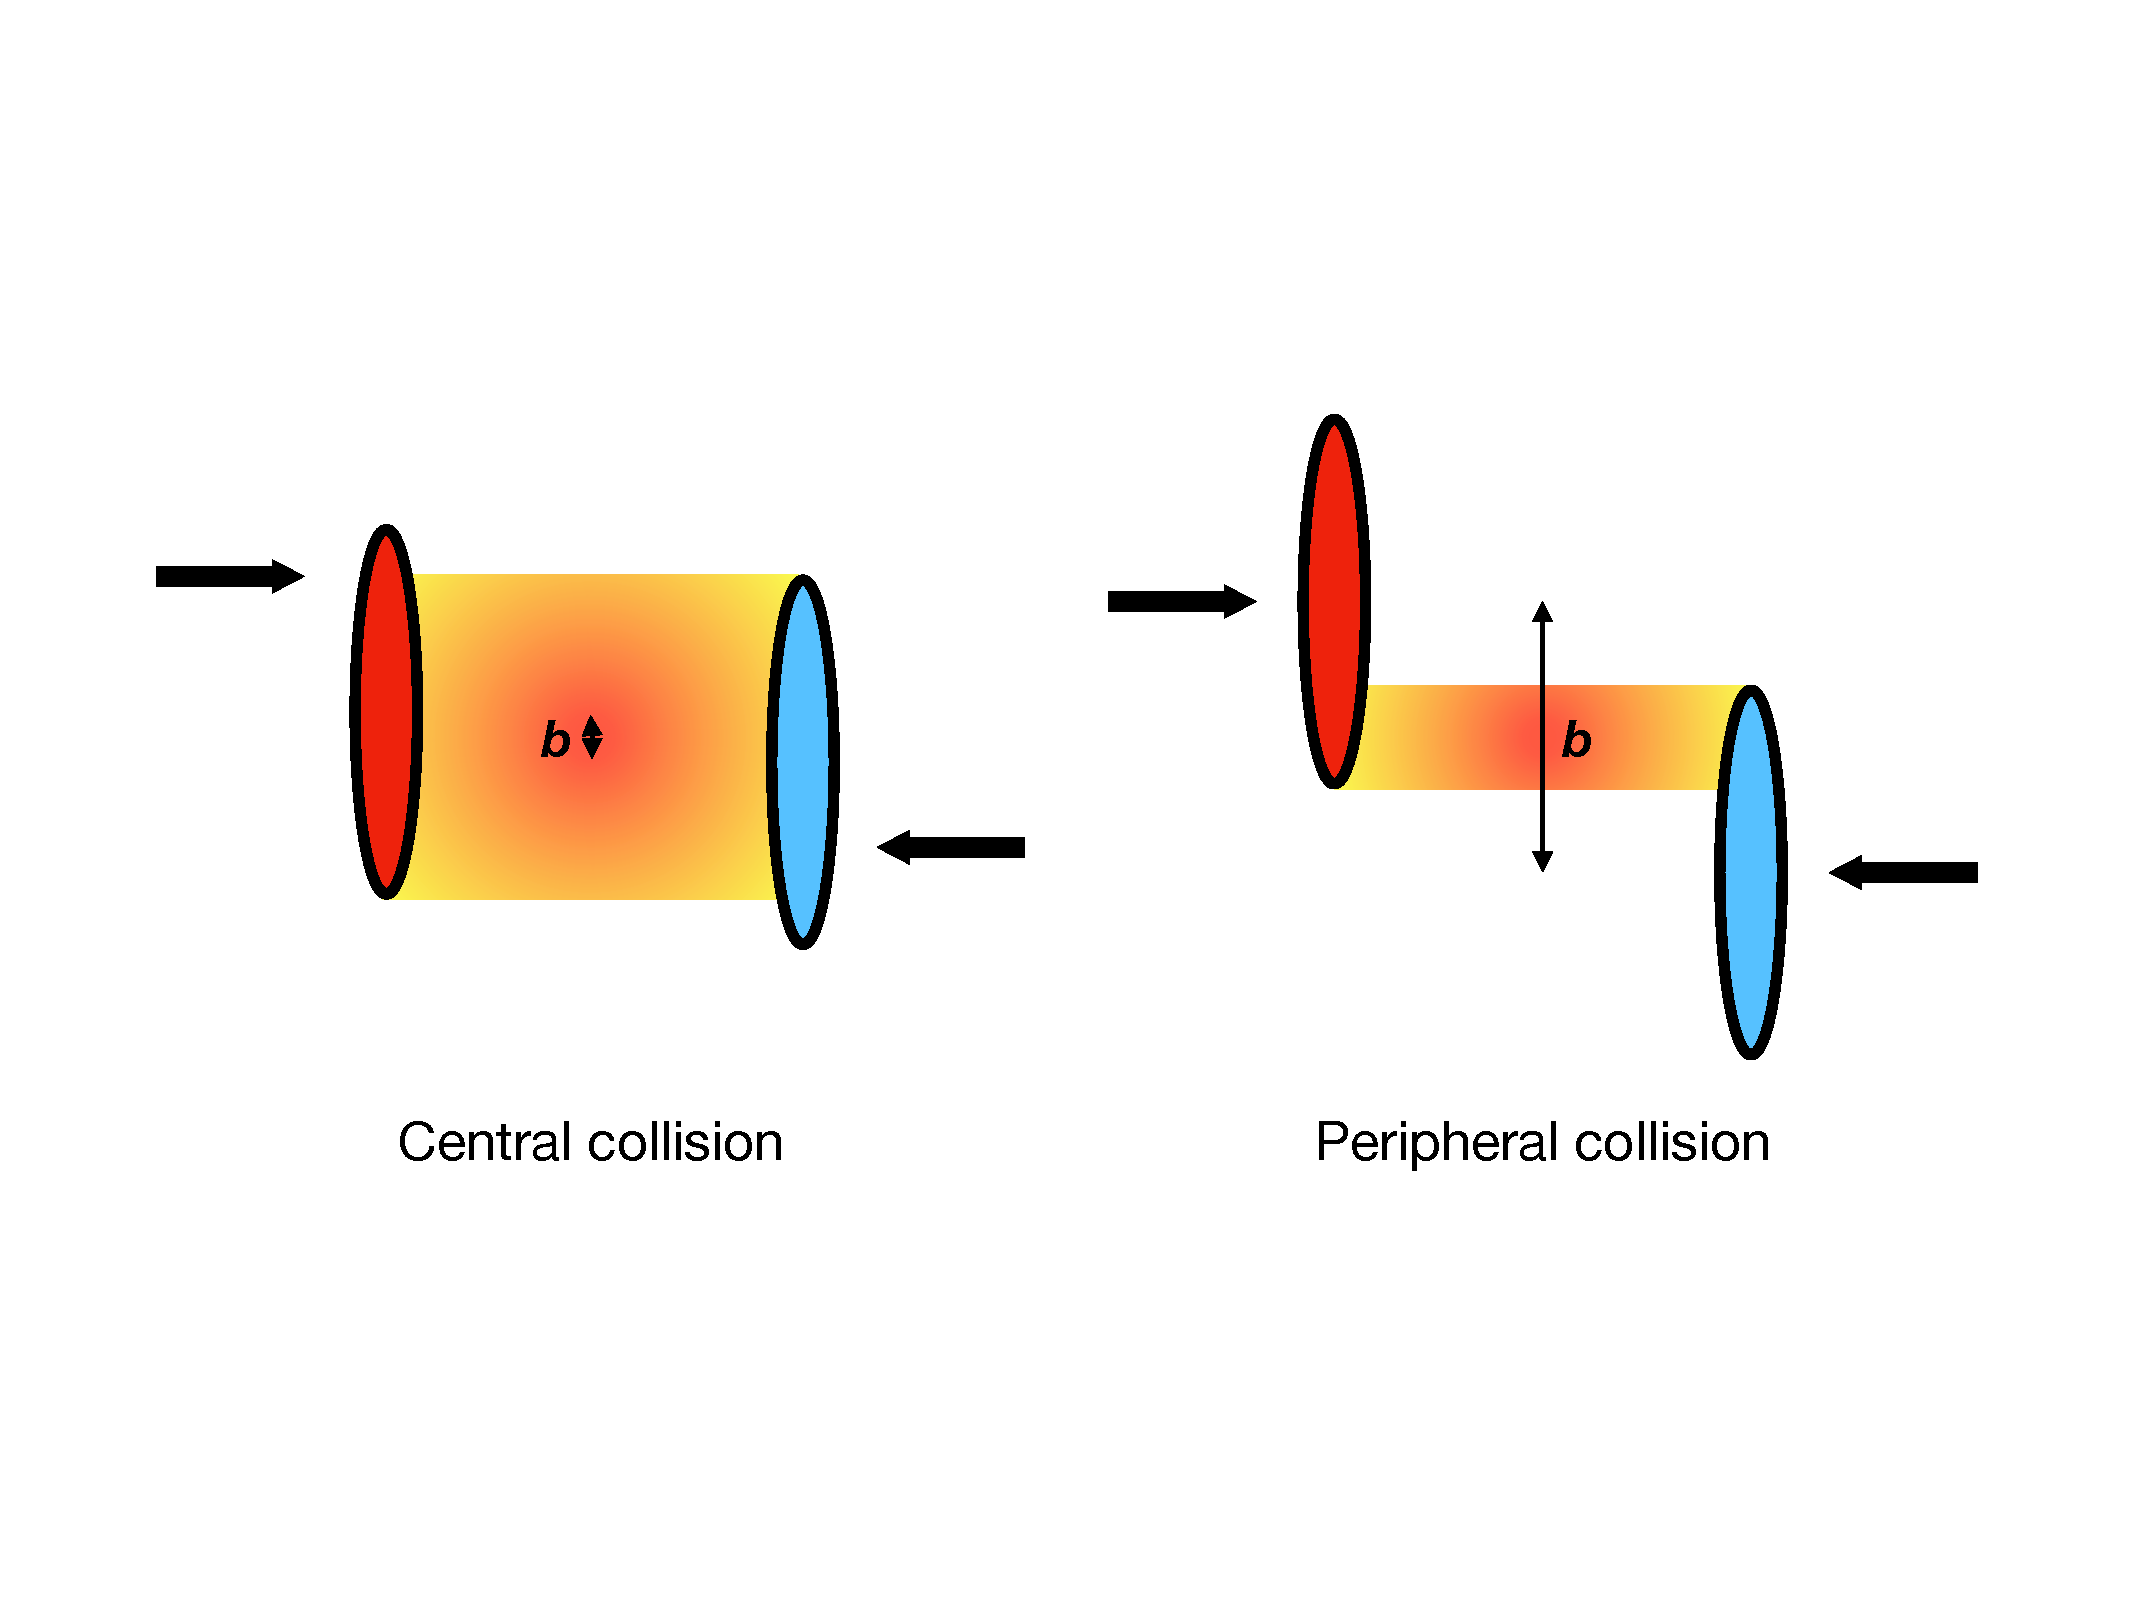
\includegraphics[width=1.\textwidth]{figures/theory/collision_centrality}
\caption{A schematic of central (left) and peripheral (right) heavy ion collisions.
The impact parameter is given by $b$.}
\label{fig:collision_centrality}
  \end{minipage}
 \qquad 
  \begin{minipage}[b]{0.45\textwidth}
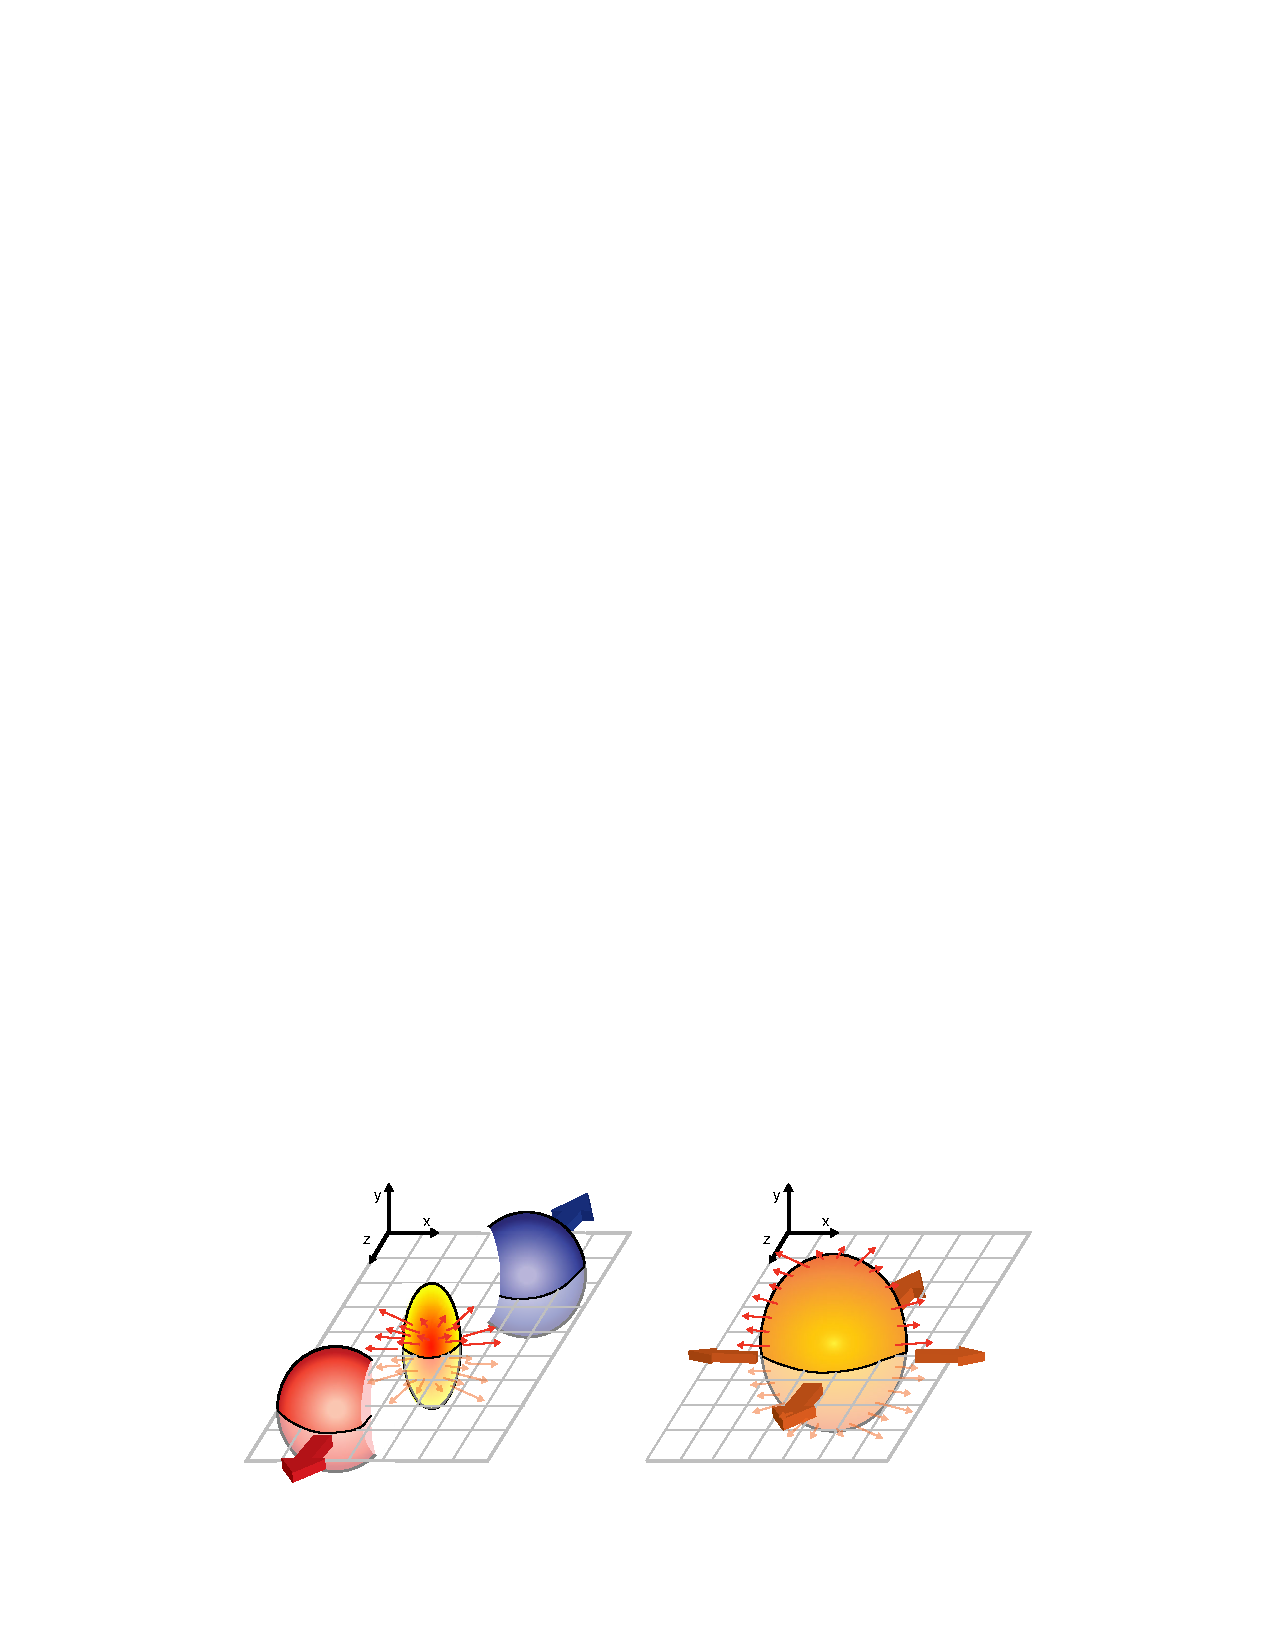
\includegraphics[width=1.\textwidth]{figures/theory/overlap}
\caption{A schematic of the initial overlap region (left) and final spatial anisotropy generated (right).
Figure from Ref.~\cite{RevModPhys.90.025005}.}
\label{fig:overlap}
\end{minipage}
\end{figure}


Properties of the QGP have been successfully described by relativistic hydrodynamic models. 
In fact, such models describing photon emission have been used to explain the data measured at both RHIC \cite{PhysRevLett.104.132301} and LHC \cite{2016235} energies and have suggested that the initial temperature of the QGP is 300--600 MeV \cite{PhysRevC.81.034911}.
The hydrodynamic nature of the QGP can be further quantified by studying the azimuthal angular distribution of particles produced in a heavy ion collision \cite{Poskanzer:1998yz, Teaney:2001av, HIRANO2006299}.
These distributions can be expanded in a Fourier series as: 

\begin{align}
\frac{d\bar{N}}{d\phi} = \frac{N}{2\pi} \left( 1 + 2 \sum_{n=1}^{\infty} v_{n} \cos(n(\phi-\Psi_n)) \right).
\end{align}
where  $N$ is the particle yield, $\phi$ is the azimuthal angle in the transverse plane and $\Psi_n$ is the orientation of the $n^{\mathrm{th}}$ order symmetry plane and is called the reaction plane.
The reaction plane, along with the participant plane, are shown in Figure~\ref{fig:reaction_plane}.
The coefficient $v_n = \langle \cos[n(\phi_i - \Psi_n)] \rangle$ is the magnitude of the $n^{\rm{th}}$ order azimuthal anisotropy, and is referred to as the flow harmonic.
The first harmonic $v_1$ is called directed flow because it indicates a particular direction, while the second harmonic $v_2$ is called elliptic flow since the azimuthal distribution in polar coordinates for $v_2 \neq 0$ is an ellipse.
These are shown in Figure~\ref{fig:flow_v1_v2}.
The azimuthal correlations that are a result of flow can be described by relativistic hydrodynamics.
A comparison of anisotropies measured in terms of $v_n$ in Ref.~\cite{ALICE:2011ab} and a hydrodynamic model described in Ref.~\cite{Niemi:2015qia} is shown in Figure~\ref{fig:flow_coeff}.


\begin{figure}
\begin{center}
  \begin{minipage}[b]{0.45\textwidth}
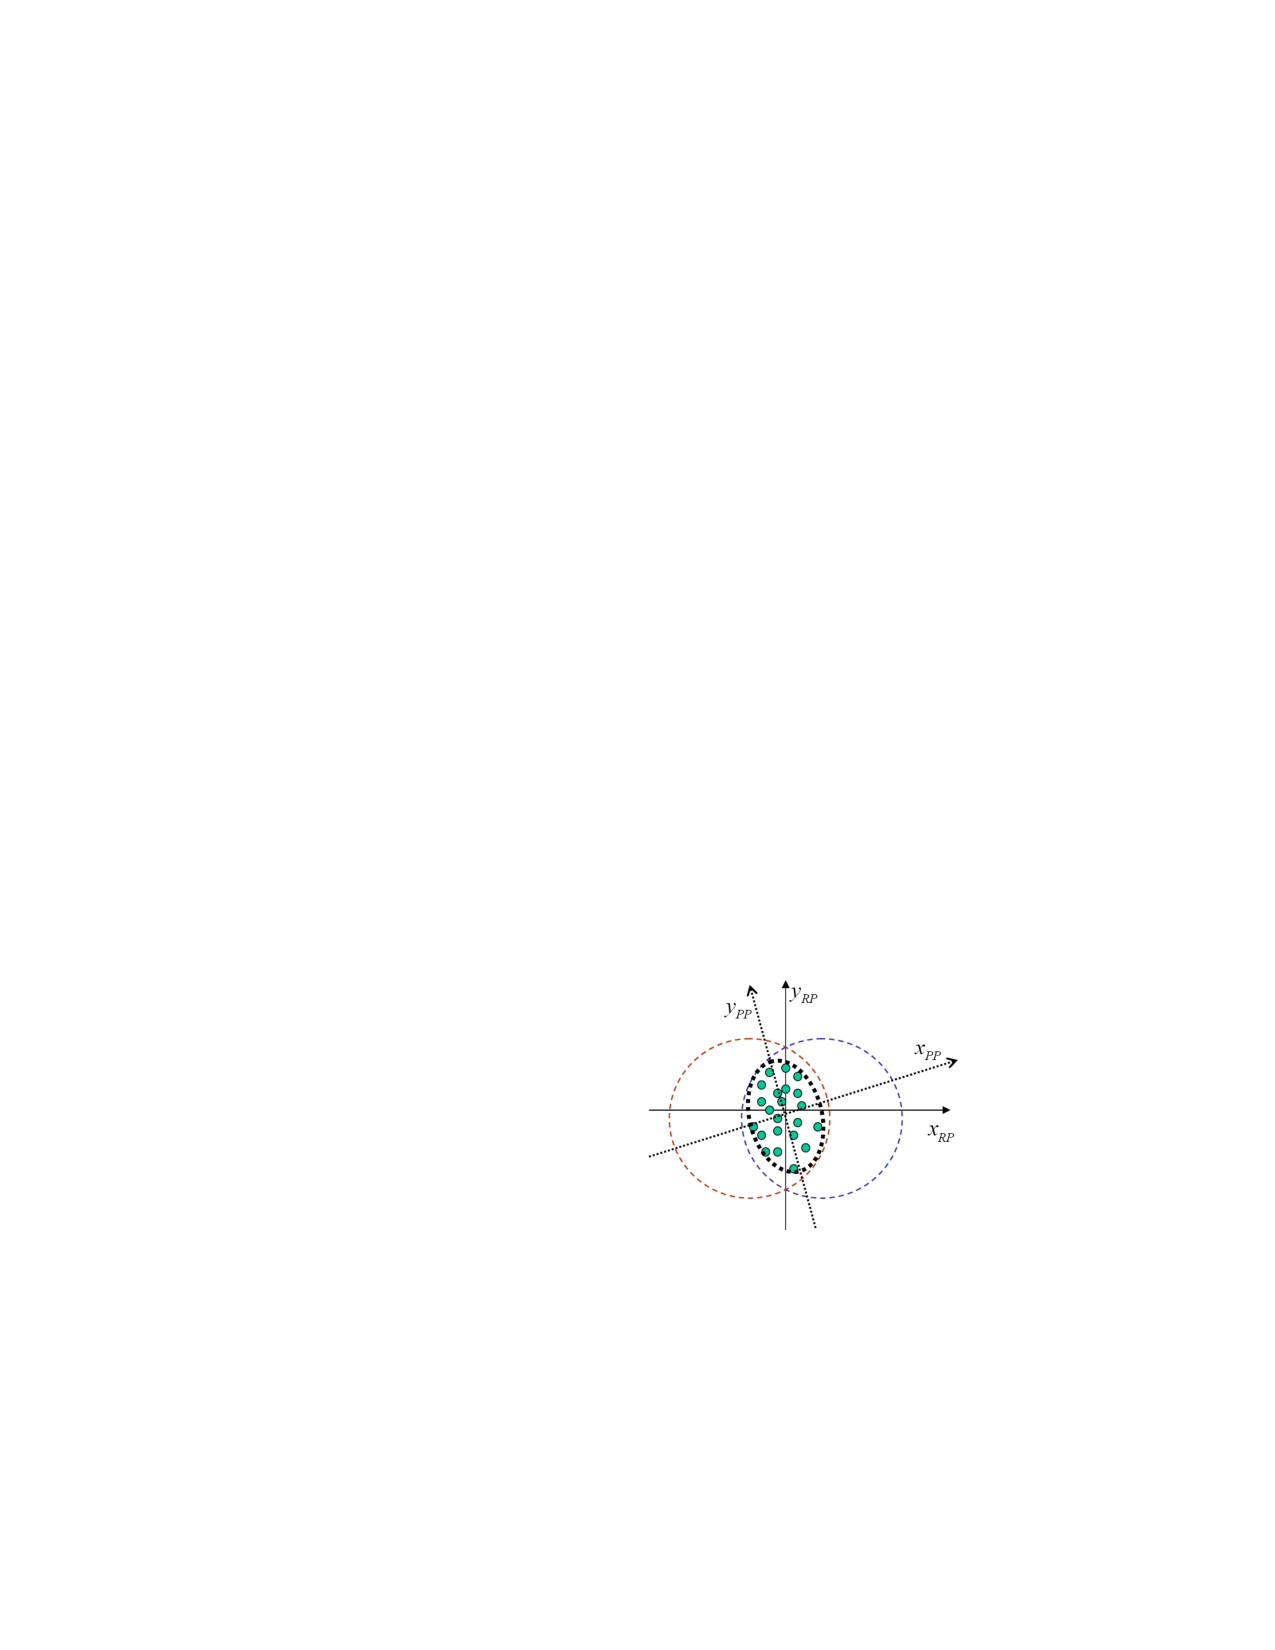
\includegraphics[width=\textwidth]{figures/theory/reaction_plane}
\caption{Definitions of the Reaction and Participant Plan coordinate systems.
Figure from Ref.~\cite{Voloshin:2008dg}.}
\label{fig:reaction_plane}
  \end{minipage}
 \qquad
 \begin{minipage}[b]{0.45\textwidth}
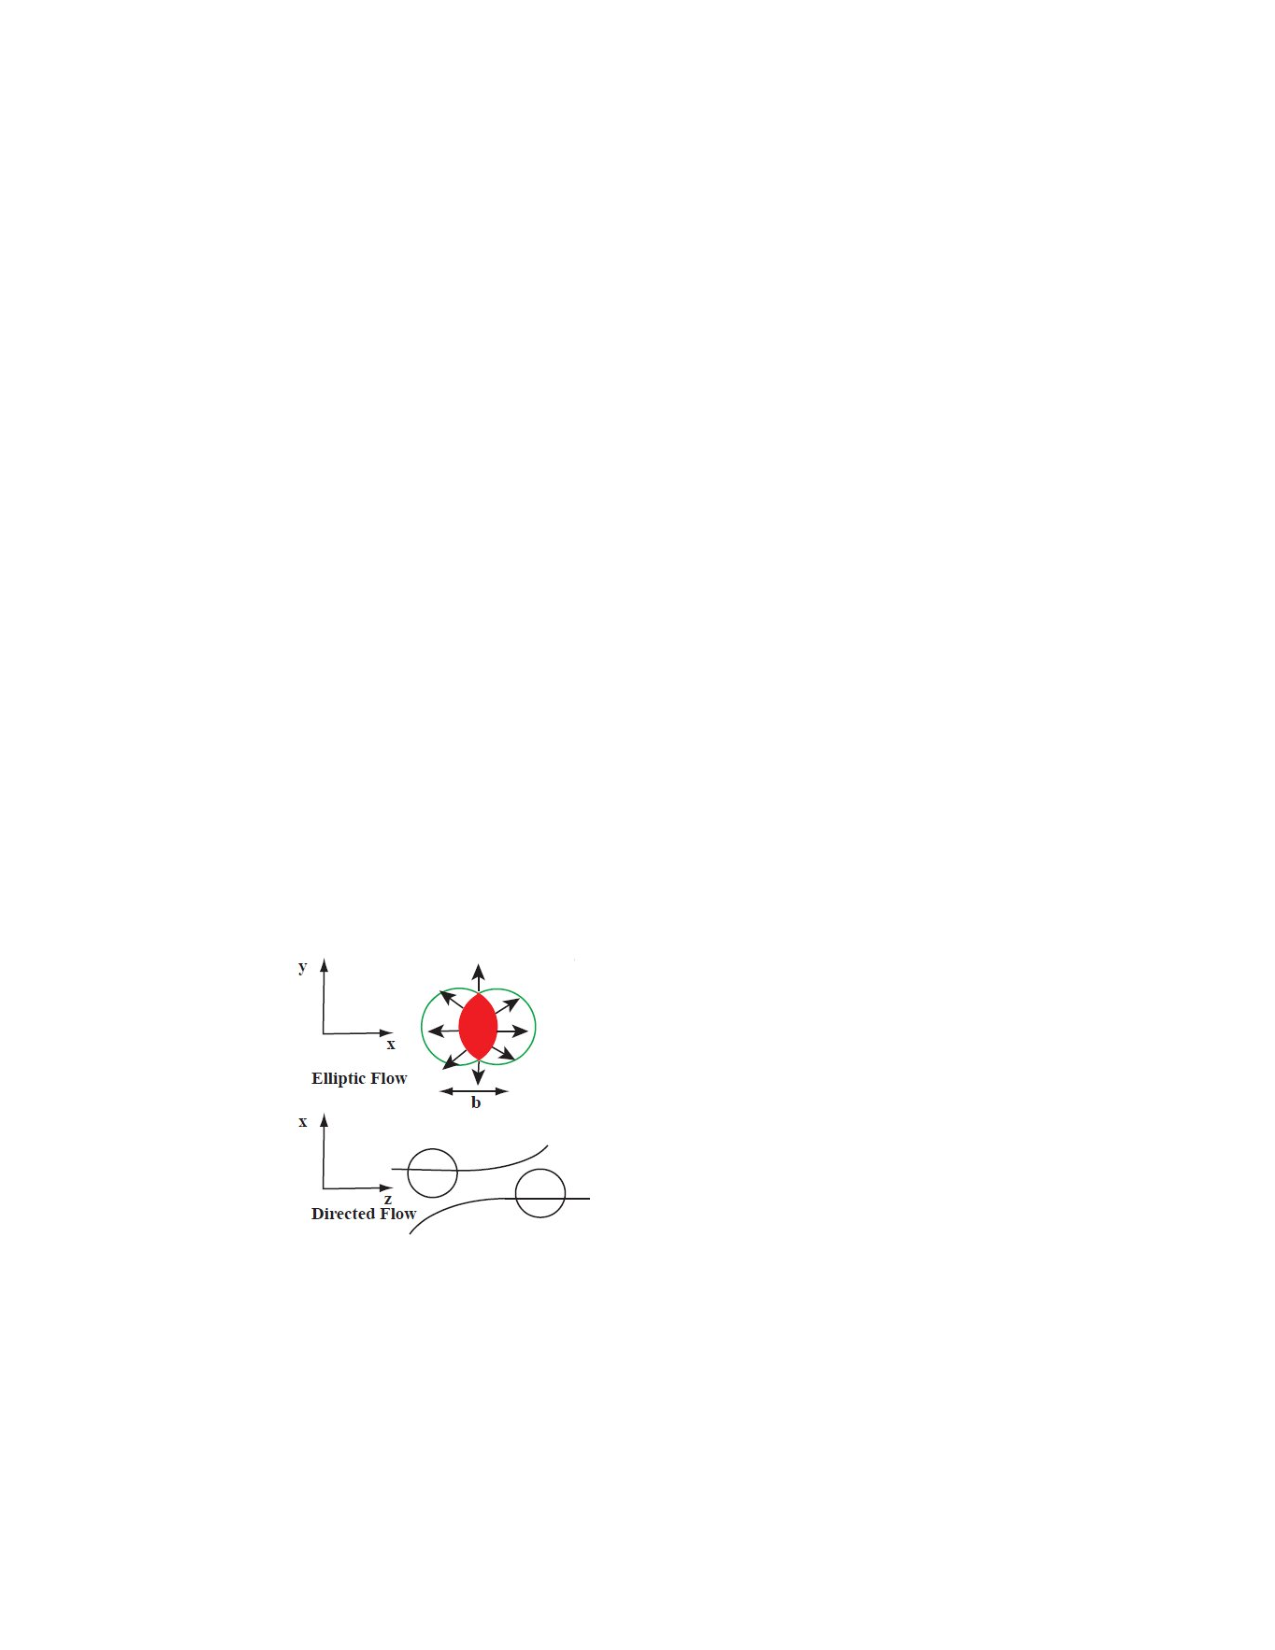
\includegraphics[width=\textwidth]{figures/theory/flow_v1_v2}
\caption{Schematics of elliptic and directed flow.
Figure from Ref.~\cite{Voloshin:2008dg}.}
\label{fig:flow_v1_v2}
  \end{minipage}
  \end{center}
\end{figure}

\begin{figure}[htbp]
\begin{center}
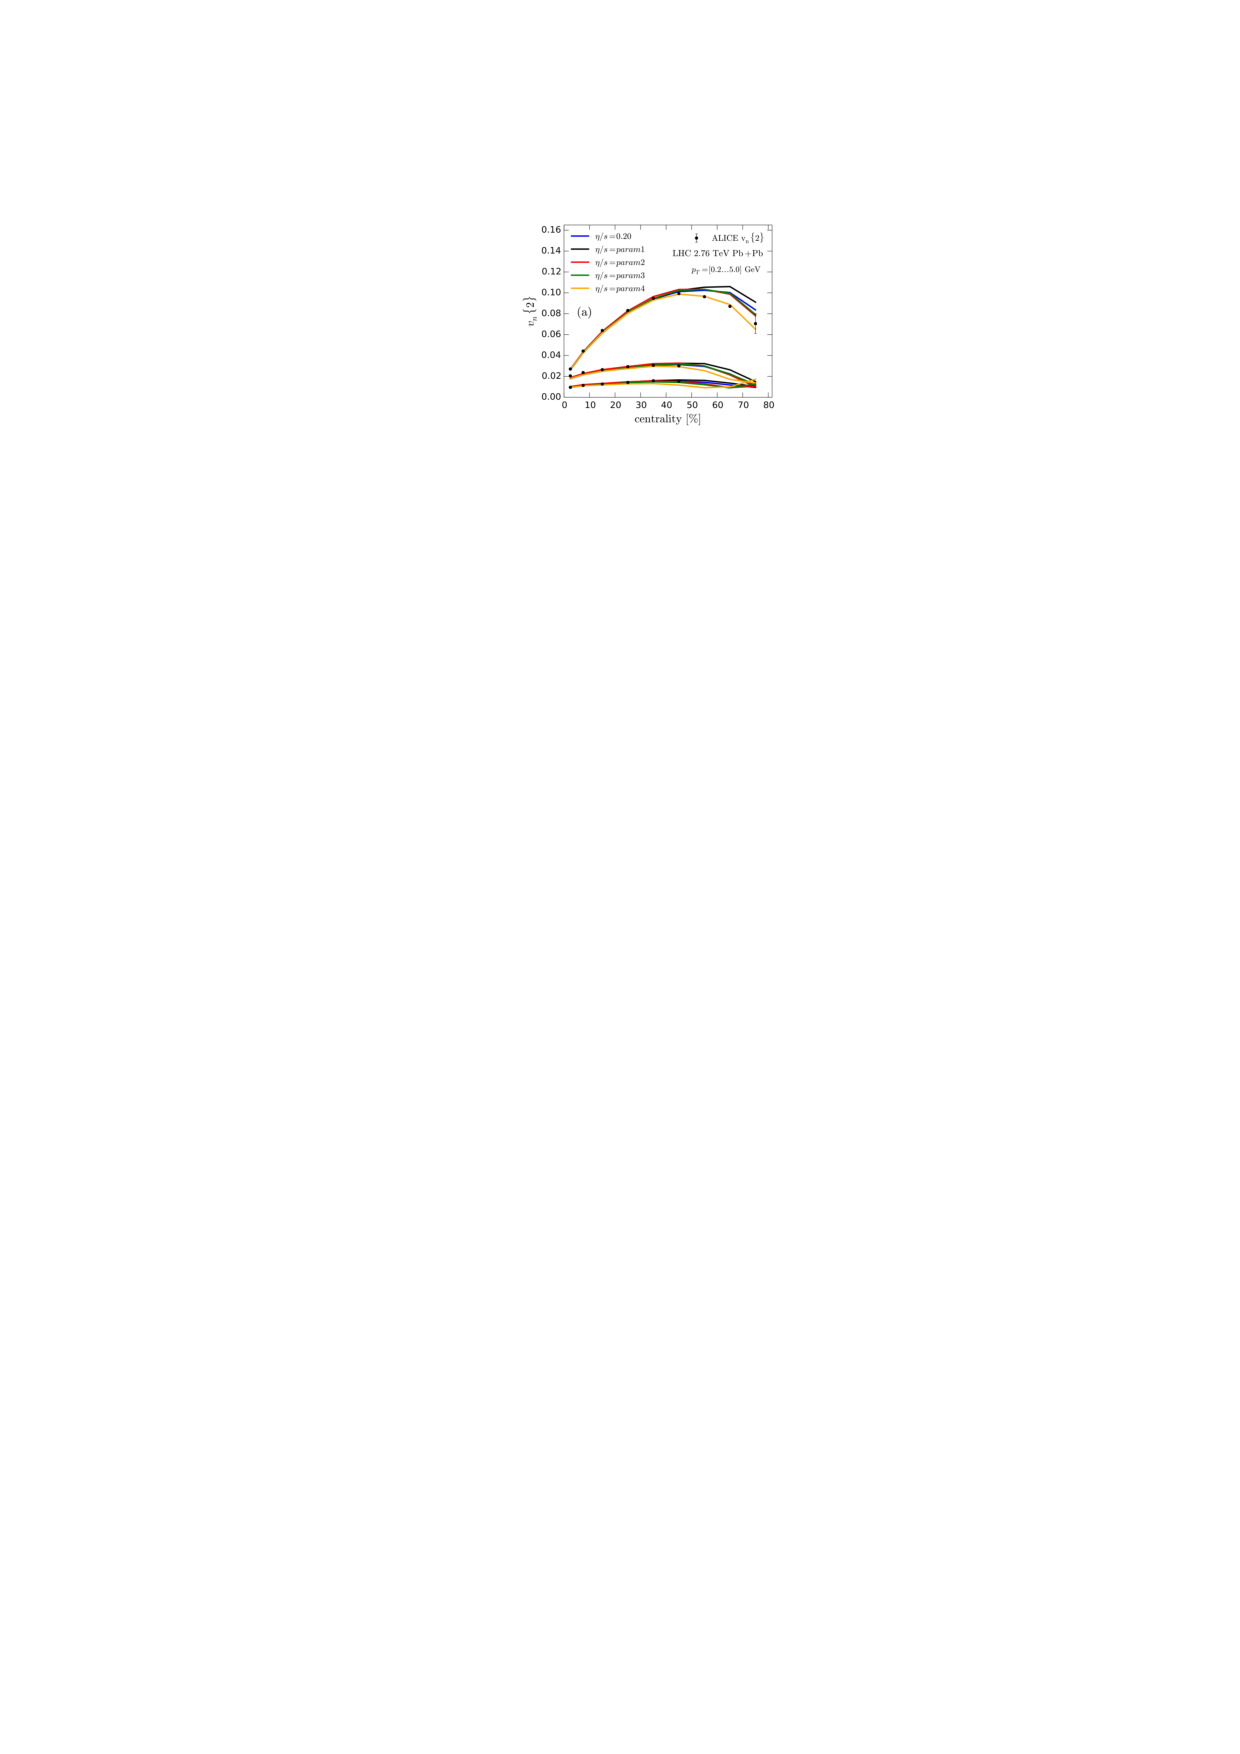
\includegraphics[width=0.45\textwidth]{figures/theory/flow_coefficients}
\caption{Comparison of a hydrodynamic model from Ref.~\cite{Niemi:2015qia} to anisotropy measurements by ALICE \cite{ALICE:2011ab} for different parameterizations of $\eta / s $ and for different $v_n$, {\it{n}} = 2, 3, 4 from top to bottom, as a function of collision centrality.
Figure from Ref.~\cite{Busza:2018rrf}.}
\label{fig:flow_coeff}
\end{center}
\end{figure}

The measured anisotropies can be used to constrain the specific viscosity given by the ratio of viscosity to entropy density, $\eta / s$, and have shown that the QGP is a near perfect liquid with an $\eta / s$ of near the theoretical minimum of $1/4\pi$ \cite{ARSENE20051, GYULASSY200530}.
In fact, this low shear viscosity is what allows the initial fluctuations in the energy density to survive the chemical freeze-out.



The thermodynamic properties of the QGP form an important field of study.
They are of particular interest since the QGP filled the early universe a few microseconds after the Big Bang \cite{PhysRevLett.34.1353}.
The QGP is also present in the core of neutron-stars \cite{Linde_1979} and the recent detection of gravitational waves from a neutron-star merger \cite{PhysRevLett.119.161101} has opened new avenues of investigation \cite{Han:2018mtj, PhysRevD.99.023009, PhysRevLett.122.061101}.
These studies have the potential to provide information into the nuclear equation of state since the dynamics of the merger are sensitive to the behavior of extremely dense nuclear matter \cite{PhysRevD.86.063001}.
The increase in temperatures and densities in merging neutron stars allows for probing different regions of the QCD phase diagram.
This is shown in Figure~\ref{fig:qcd_phase} as a function of temperature $T$ and baryon chemical potential $\mu$.
In particular, differences in gravitational-waves from these systems before and after the merger can be used to provide an observable signature of a first order phase transition \cite{PhysRevLett.122.061102}.
Colliders like RHIC and the LHC on the other hand probe regions that have near zero low baryon densities, where the transition is a smooth crossover that spans a 20--30 MeV temperature range.


\begin{figure}[htbp]
\begin{center}
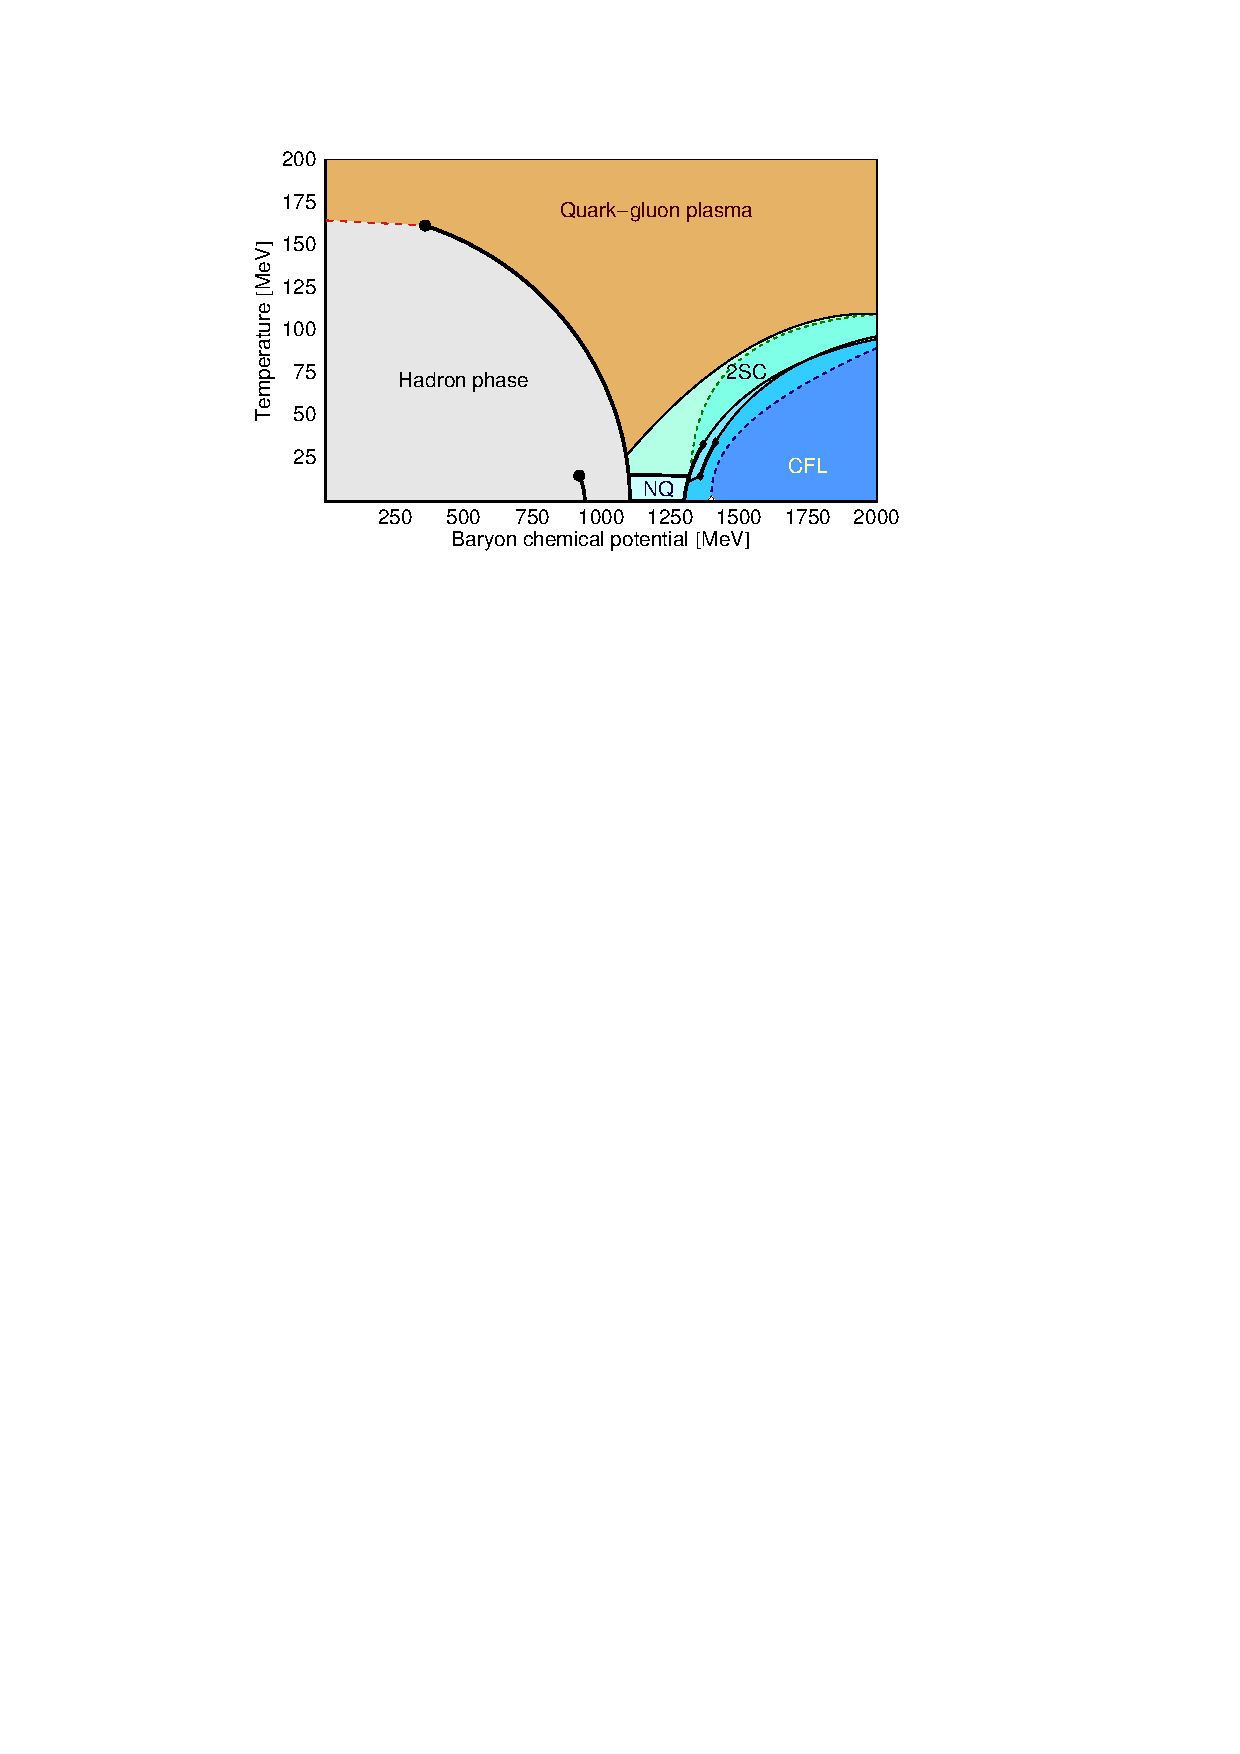
\includegraphics[width=0.45\textwidth]{figures/theory/qcd_phase}
\caption{The QCD phase diagram of nuclear matter as a function of temperature $T$ and baryon chemical potential $\mu$.
The $n\star$ denotes a neutron star.
Figure from Ref.~\cite{Kronfeld:2012uk}.}
\label{fig:qcd_phase}
\end{center}
\end{figure}


\subsection{The Glauber Model}
The basic parameters of a heavy ion collision such as the number of participants \Npart\ and number of binary collisions \Ncoll\ can be determined using the Glauber Monte Carlo simulations \cite{glauberArticle}.
This technique considers a nucleus-nucleus collision as a collection of independent binary nucleon-nucleon collisions; the colliding nuclei are modeled as a set of uncorrelated nucleons being positioned within the nucleus based on a the nuclear density function uniform in azimuthal and in polar angles.
The nuclear density function in this model is a Woods-Saxon distribution given by: 

\begin{align}
\rho(r) = \rho_0 \frac{1 + w (r/R)^2}{1+e^{\frac{r-R}{a}}}
\end{align}
where $\rho_0$ is the nucleon density, $R$ is the nuclear radius, $a$ is the skin depth, $w$ corresponds to deviations from a circular shape and is typically zero for larger nuclei like Cu, W, Au, Pb, and U.
For the Pb nuclei used at the LHC, $w = 0$, $R = 6.62$ fm and $a =0.55$ fm \cite{DEVRIES1987495}.
The nuclear density distribution for Au and Cu is shown in Figure~\ref{fig:nuclearDensity}.

\begin{figure}[htbp]
\begin{center}
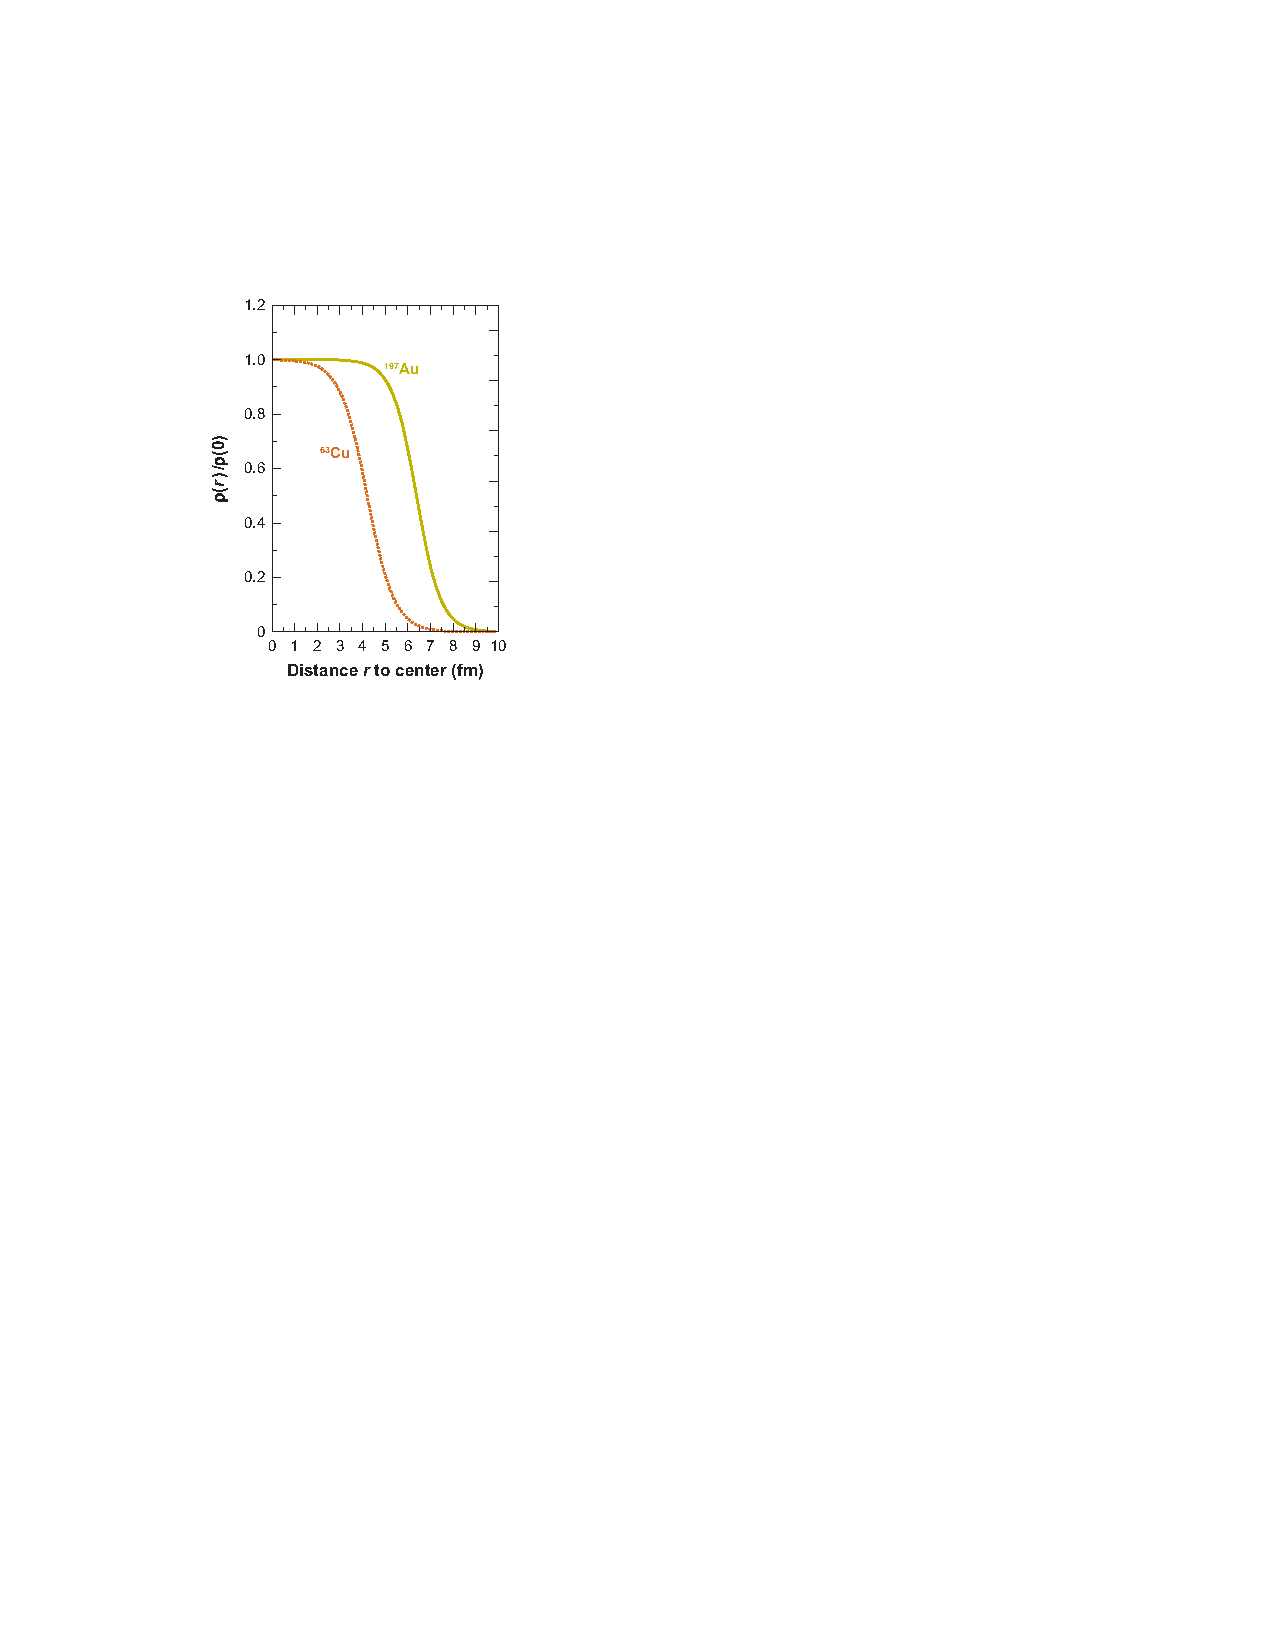
\includegraphics[width=0.35\textwidth]{figures/theory/nuclearDensity}
\caption{ The nuclear density distributions for nuclei used at RHIC: Cu ($w = 0$, $R = 4.2$ fm and $a =0.48$ fm)  and Au ($w = 0$, $R = 6.38$ fm and $a =0.535$ fm) \cite{DEVRIES1987495}.
Figure from Ref.~\cite{doi:10.1146/annurev.nucl.57.090506.123020}.}
\label{fig:nuclearDensity}
\end{center}
\end{figure}

They are then arranged with a random impact parameter $b$ based on the distribution $d\sigma/d b = 2\pi b$ and projected onto the $x-y$ plane as shown in Figure~\ref{fig:glauberMC}.
They are then made to travel on straight trajectories, colliding if $d \leq \sqrt{\sigma_{\mathrm{inel}}^{\mathrm{NN}}/ \pi}$, where $d$ is the distance between the nucleons in a plane transverse to the beam axis and $\sigma_{\mathrm{inel}}^{\mathrm{NN}}$ is the inelastic scattering cross section \cite{doi:10.1146/annurev.nucl.57.090506.123020, Alver:2008aq}.


\begin{figure}[htbp]
\begin{center}
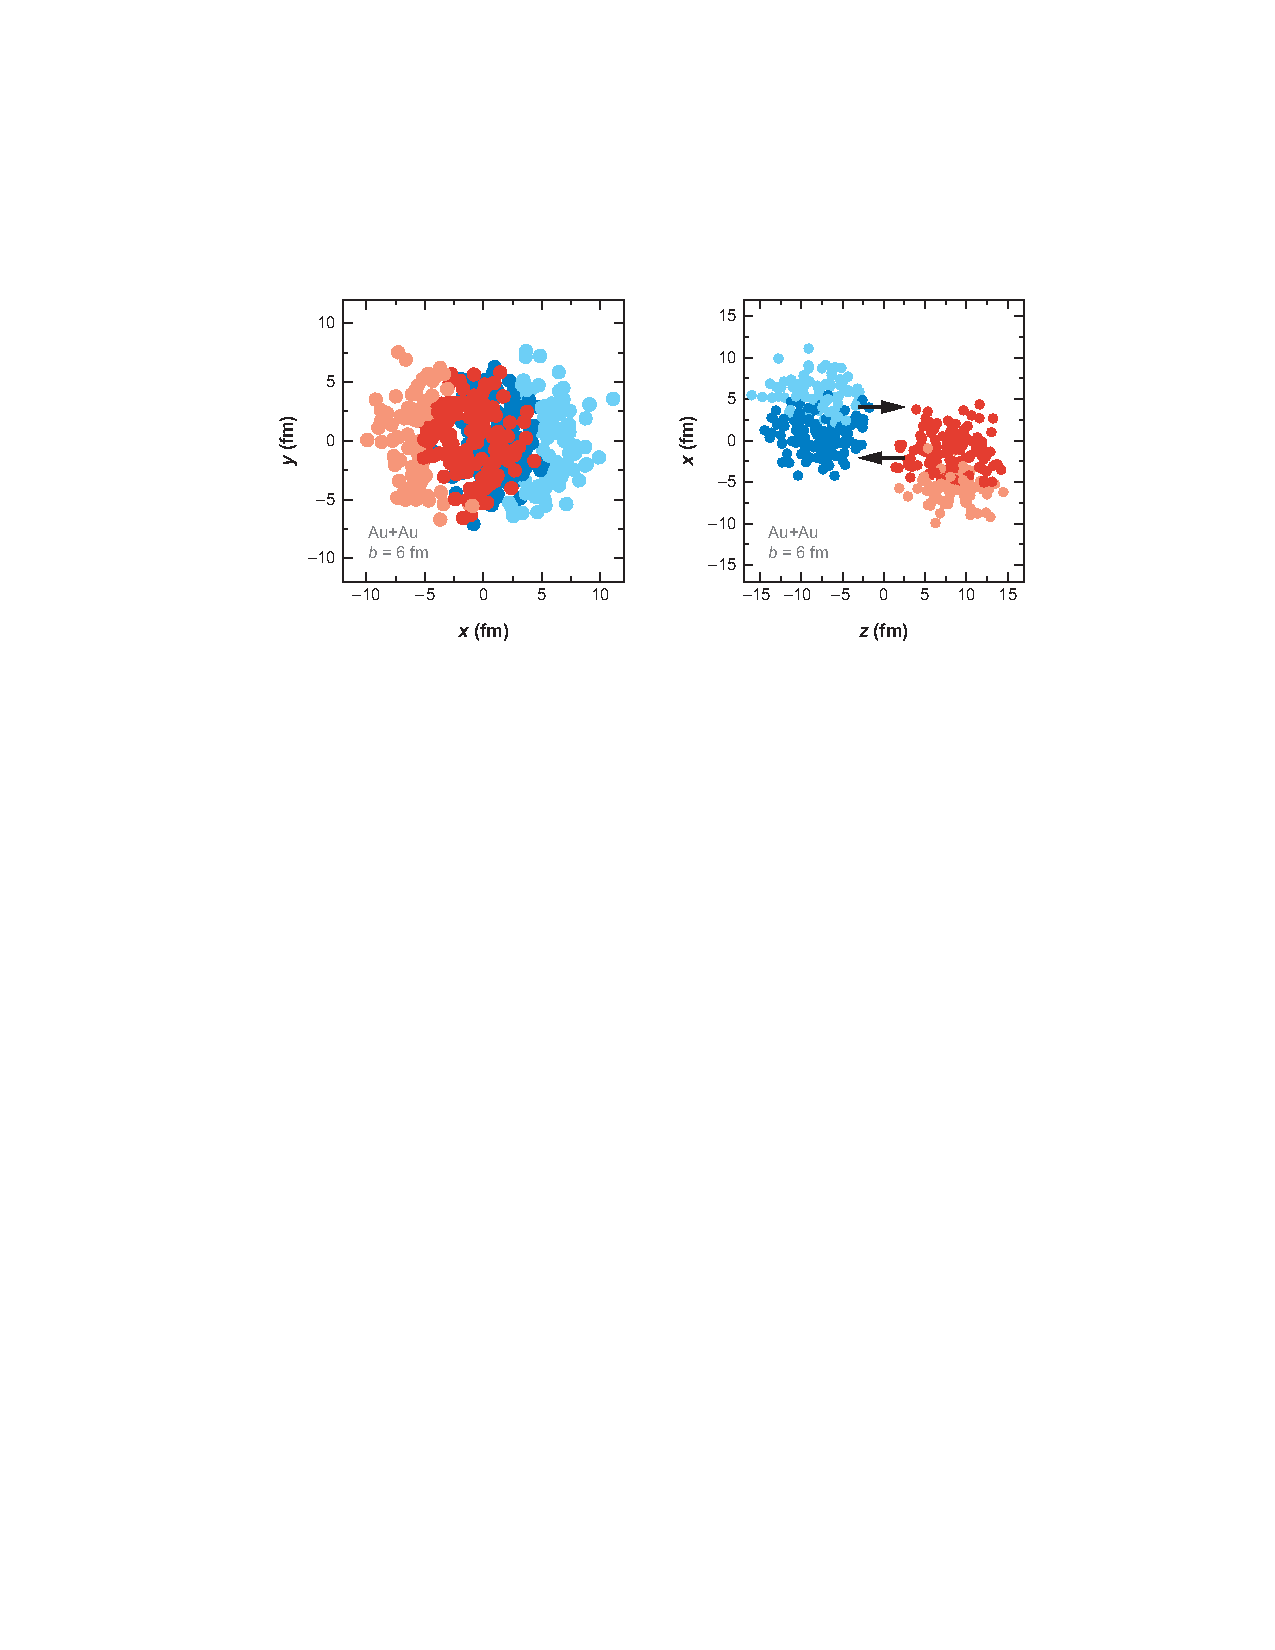
\includegraphics[width=0.85\textwidth]{figures/theory/glauberMC}
\caption{A Glauber Monte Carlo event for $Au+Au$ at \sqrtsnn = 200 geV with impact parameter of 6 fm viewed in the (left) transverse plane and (right) along the beam axis.
Darker circles represent the participating nucleons.
Figure from Ref.~\cite{doi:10.1146/annurev.nucl.57.090506.123020}.}
\label{fig:glauberMC}
\end{center}
\end{figure}

An important parameter for colliding nuclei A and B with $A$ and $B$ nucleons is the thickness function $T_{AB}$.
It describes the effective overlap area in which specific nucleons in the two colliding nuclei can interact.
It can be defined in terms of the probability per unit area of a given nucleon being located at a particular distance $s$ within the nucleus.
For the colliding nuclei $A$ and $B$, this is given by $T_{A}({\bf{s}}) = \int \rho_A ({\bf{s}}, z_A) dz_{A}$ and $T_{B}({\bf{s}}) = \int \rho_B ({\bf{s}}, z_B) dz_{B}$.
Then, $T_{AB}$ is given by

\begin{align}
T_{AB}({\bf b}) = \int T_{A} ({\bf s}) T_{B} ({\bf s-\bf b}) d^2 s
\end{align}
The probability of then having $n$ interactions between nuclei $A$ and $B$ is given by the binomial distribution:

\begin{align}
P(n, { \bf b}) = {{AB} \choose {n}} \Big[T_{AB}( {\bf b} ) \sigma_{\mathrm{inel}}^{\mathrm{NN}} \Big]^n \Big[ 1 - T_{AB}( {\bf b} ) \sigma_{\mathrm{inel}}^{\mathrm{NN}} \Big]^{AB-n}
\end{align}
where the first term is the number of combinations for finding $n$ collisions from $AB$ possibilities, the second term is the probability for having exactly $n$ collisions, and the last term the probability of $AB-n$ misses.
Then the total probability of an interaction between A and B is:

\begin{align}
\frac{d^2  \sigma_{\mathrm{inel}}^{\mathrm{AB}} }{db^2} \equiv p_{\mathrm{inel}}^{\mathrm{AB}} (b) = \sum_{n=1}^{AB} P(n, {\bf b}) = 1- \Big[ 1 - T_{AB}( {\bf b} ) \sigma_{\mathrm{inel}}^{\mathrm{NN}} \Big]^{AB}
\end{align}
and the total cross section is given by

\begin{align}
\sigma_{\mathrm{inel}}^{\mathrm{AB}} = \int_0^\infty 2\pi b db \Bigg[ 1- \Big( 1 - T_{AB}( {\bf b} ) \sigma_{\mathrm{inel}}^{\mathrm{NN}}  \Big)^{AB} \Bigg]
\end{align}
and \Ncoll\ and \Npart are given by \cite{Kharzeev:2000ph, Bialas:1976ed}:

\begin{align}
\Ncoll (b) = & \sum_{n=1}^{AB} n P(n, b) =  AB \times T_{AB}(b) \sigmainel \\
\Npart (b) = & A \int T_A ({\bf s}) \Big[ 1 - \big(1-T_B ({\bf s - b}) \sigmainel \big)^B \Big] d^2 s \\
+ & B \int T_B ({\bf s-b}) \Big[ 1 - \big(1-T_A ({\bf s}) \sigmainel \big)^A \Big] d^2 s \nonumber
\end{align}
The correlation between \Ncoll\ and \Npart\ can be seen in Figure~\ref{fig:NcollNpart}.
The charged particle multiplicity $N_{\mathrm{ch}}$ along with the combination of \Npart\ and impact parameter $b$ can be used to determine the centrality of a heavy ion event.
An example of this is shown in Figure~\ref{fig:cent_estimate}.

\begin{figure}
\begin{center}
  \begin{minipage}[b]{0.4\textwidth}
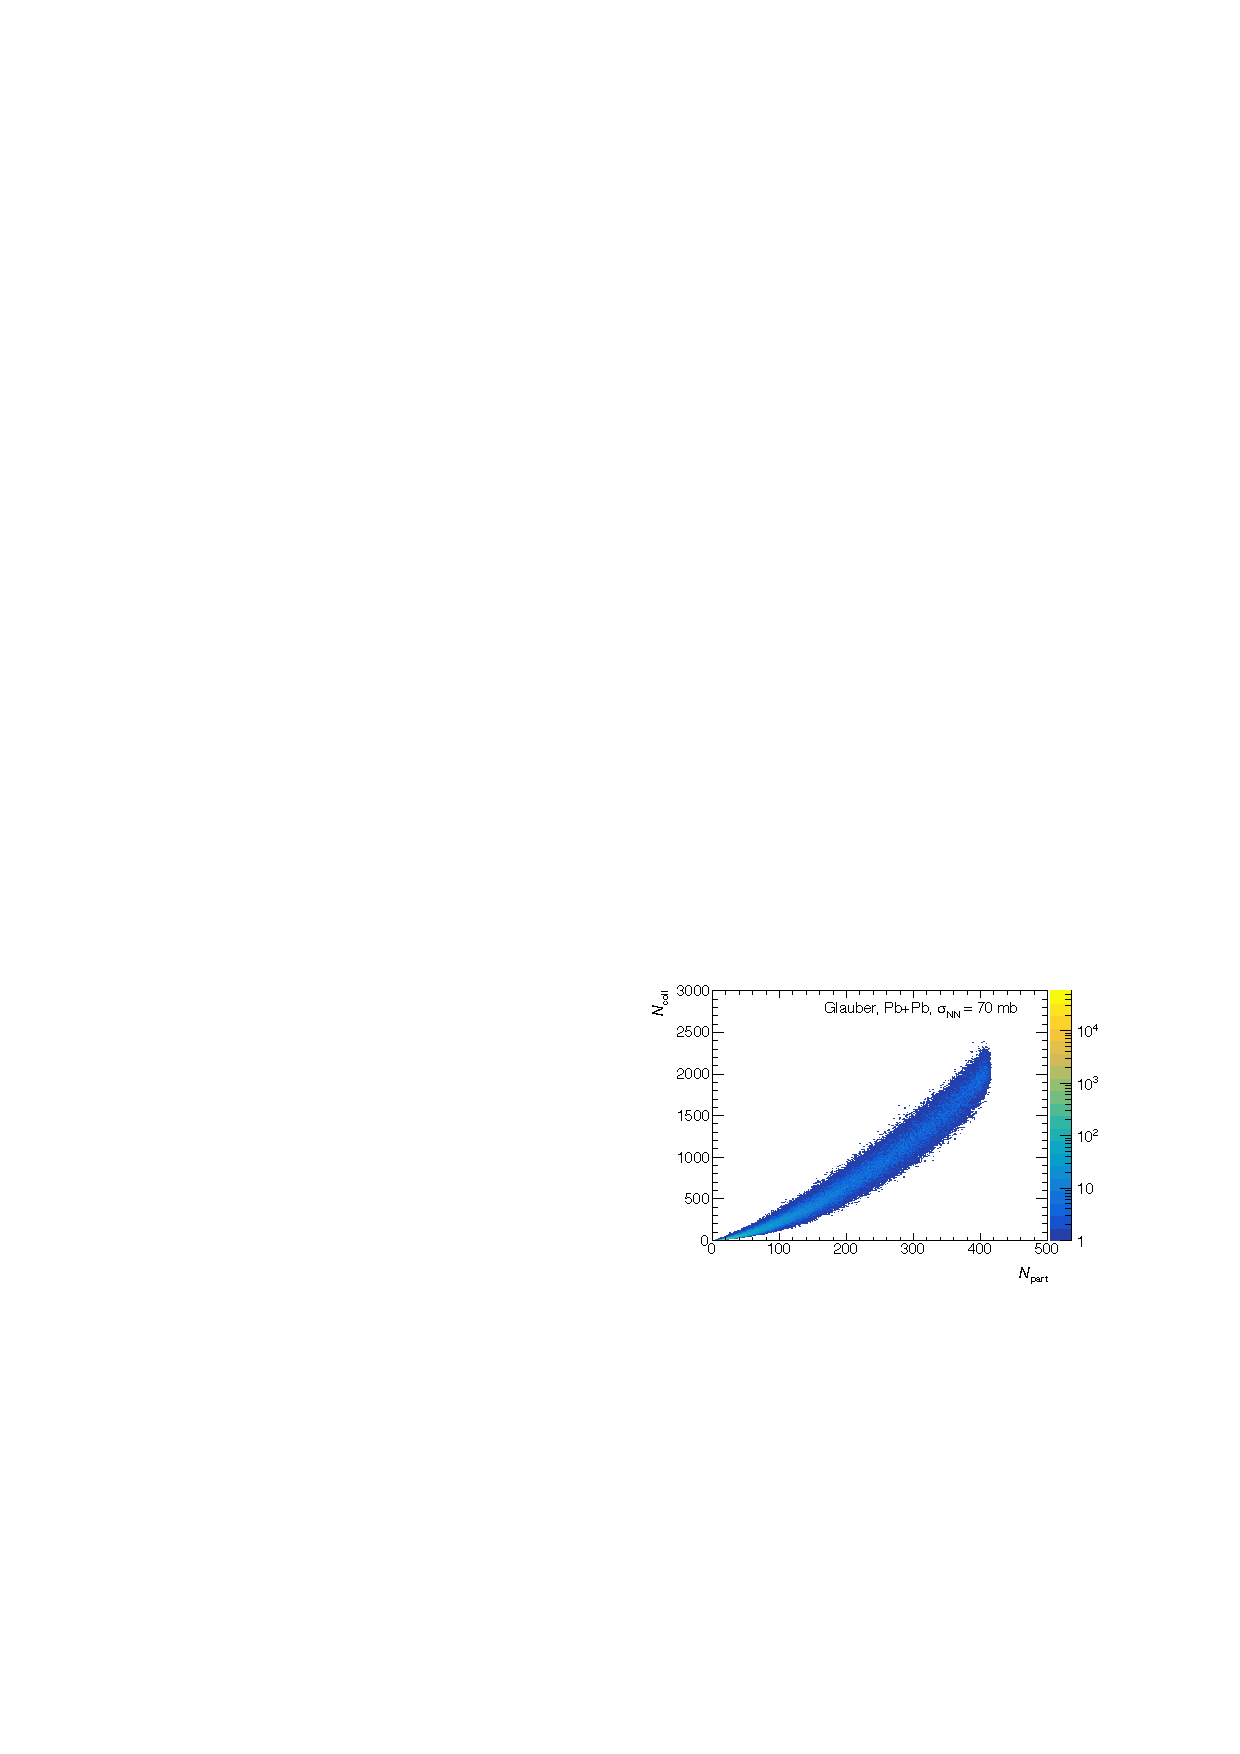
\includegraphics[width=\textwidth]{figures/theory/NcollNpart}
\caption{The $\Ncoll-\Npart$ correlation for \pbpb\ collisions at \sqrtsnn\ = 5.02 TeV.
Figure from Ref.~\cite{Perepelitsa:2212936}.}
\label{fig:NcollNpart}
  \end{minipage}
 \qquad  \qquad  \qquad
  \begin{minipage}[b]{0.4\textwidth}
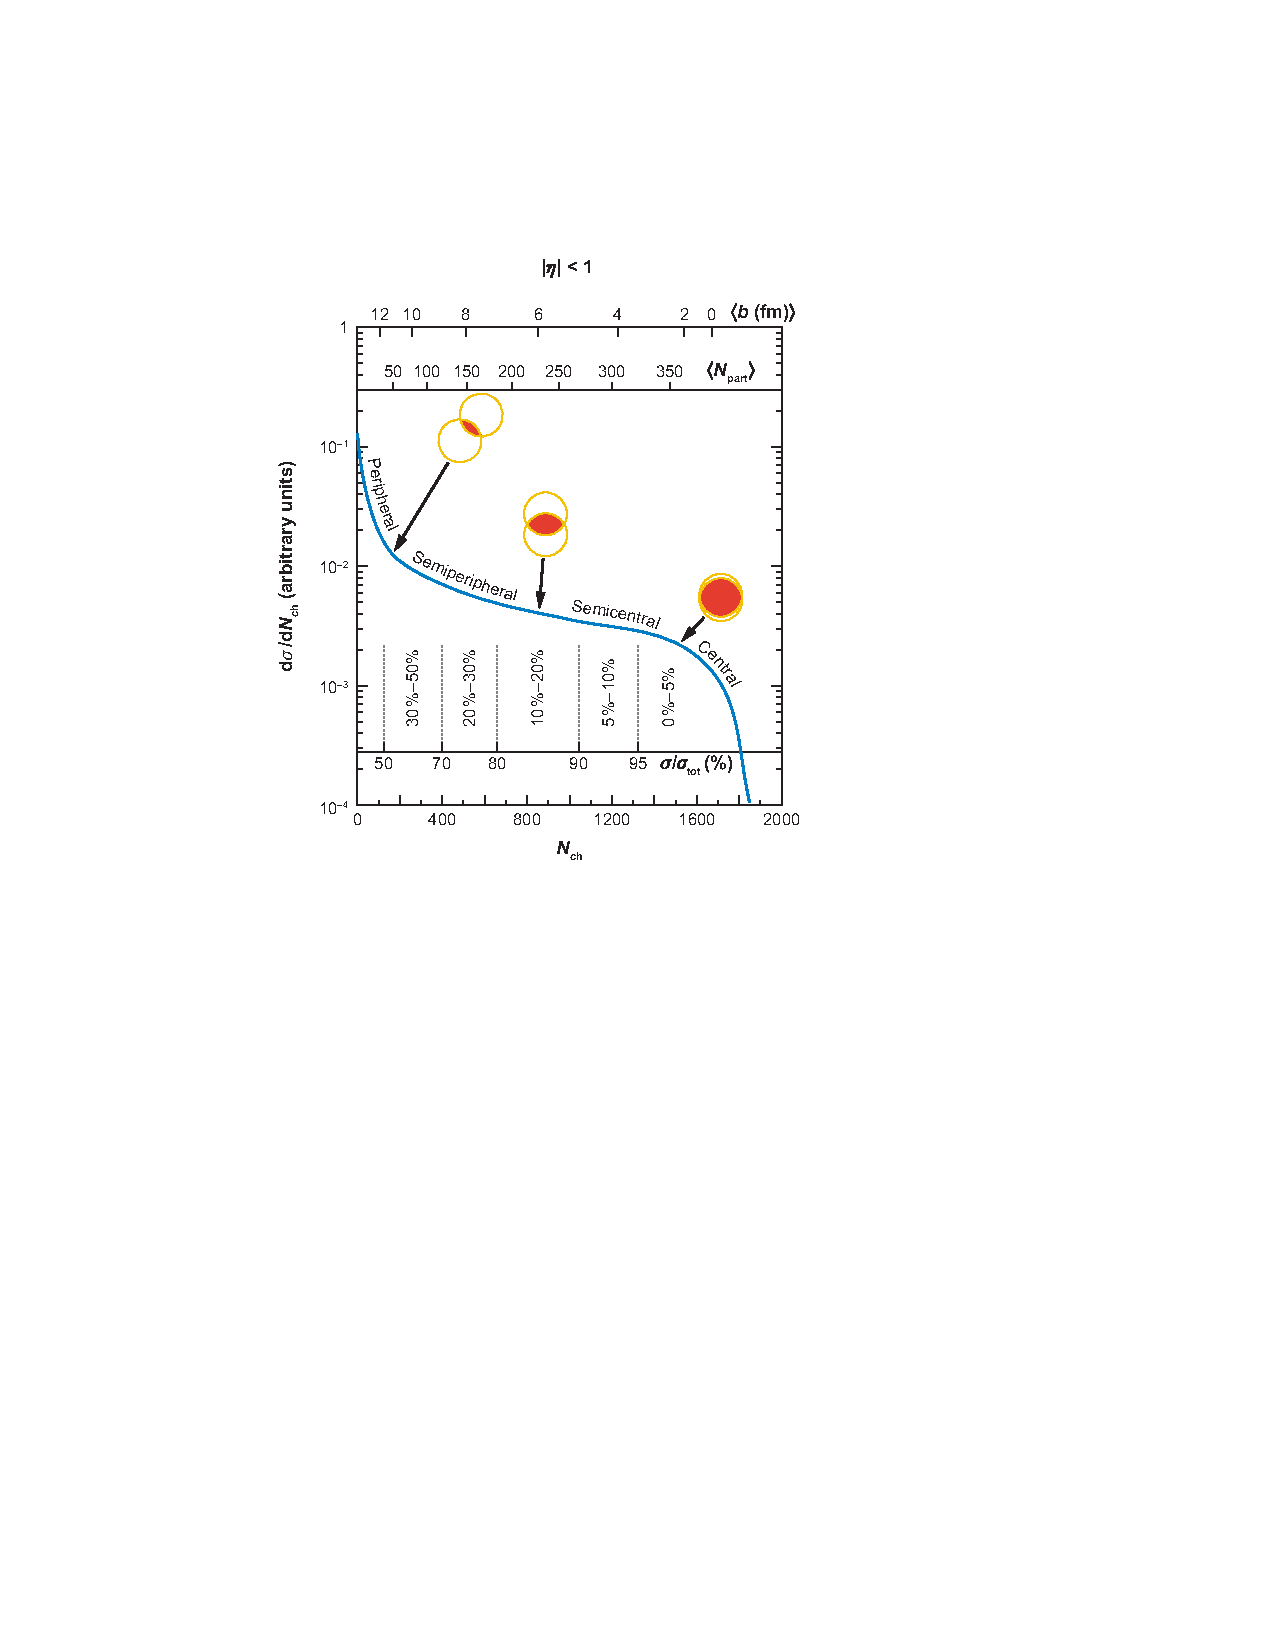
\includegraphics[width=\textwidth]{figures/theory/cent_estimate}
\caption{The correlation between the observable \Nch\ and \Npart\ to determine the centrality distribution.
Figure from Ref.~\cite{doi:10.1146/annurev.nucl.57.090506.123020}.}
\label{fig:cent_estimate}
  \end{minipage}
  \end{center}
\end{figure}





%Hydrodynamic models of photon emission can be used to describe data measured at both RHIC \cite{PhysRevLett.104.132301} and LHC \cite{2016235} energies and suggest that the initial temperature of the QGP is 300--600 MeV \cite{PhysRevC.81.034911}.
%Each nucleus contains many colored quarks and antiquarks, with three more quarks than anti-quarks per nucleon, with the $q\bar{q}$ popping in and out of the vacuum due to quantum fluctuations.
%These $q\bar{q}$ pairs are sources of transverse color fields and the corresponding force carriers, the gluons.
%Lattice QCD calculations in these regions show that the transition between a hadronic gas and the QGP occurs at a temperature of approximately 160 MeV and corresponds to an energy density of 0.5 GeV/fm$^3$ \cite{Borsanyi:2010bp}.
%Heavy ion collisions are a tool that can be used as a tool to study the quark-gluon plasma (QGP) \cite{SHURYAK198071}.